% This is a template for students in MATH 3000 at FSU to formally write-up results presented in class. 

% All of this stuff with '%' in front is a comment and ignored by the compiler.
%
% The lines before the "\begin{document}" line is called the preamble.
% This is where you load particular packages you need.
% Until you are more experienced, or the program says you are missing packages, it is safe to ignore most of the preamble.
%
%----------------------------------

\documentclass[12pt]{article}
\usepackage[margin=1in]{geometry}% Change the margins here if you wish.
\setlength{\parindent}{0pt} % This is the set the indent length for new paragraphs, change if you want.
\setlength{\parskip}{5pt} % This sets the distance between paragraphs, which will be used anytime you have a blank line in your LaTeX code.
\pagenumbering{gobble}% This means the page will not be numbered. You can comment it out if you like page numbers.

\usepackage{listings}
\usepackage[export]{adjustbox}
\usepackage{subcaption}

%------------------------------------

% These packages allow the most of the common "mathly things"
\usepackage{amsmath,amsthm,amssymb}

% This package allows you to add images.
\usepackage{graphicx}
\usepackage{float}

% These are theorem environments.  This should cover everything you need, and you should be able to tell what environment goes with what type of result, but please let me know if I've missed anything.
\newtheorem{euclidtheorem}{Proposition}
\newtheorem{classtheorem}{Theorem}
\newtheorem{theorem}{Theorem}[section]
\newtheorem{challenge}[theorem]{Challenge}
\newtheorem{question}[theorem]{Question}
\newtheorem{problem}[theorem]{Problem}


\newtheorem{theorempiece}{Theorem}[theorem]
\newtheorem{classtheorempiece}{Theorem}[classtheorem]
\newtheorem{challengepiece}{Challenge}[theorem]
\newtheorem{questionpiece}{Question}[theorem]
\newtheorem{problempiece}{Problem}[theorem]

%These help to format the names of the results the way we are in class and in notes.
\renewcommand*{\theeuclidtheorem}{\Roman{section}.\arabic{theorem}}
\renewcommand*{\thetheorem}{\arabic{section}.\arabic{theorem}}
\renewcommand*{\theclasstheorem}{\Alph{theorem}}
\renewcommand*{\thechallenge}{\arabic{section}.\arabic{theorem}}
\renewcommand*{\thequestion}{\arabic{section}.\arabic{theorem}}
\renewcommand*{\theproblem}{\arabic{section}.\arabic{theorem}}
\renewcommand*{\thetheorempiece}{\arabic{section}.\arabic{theorem}.\alph{theorempiece}}
\renewcommand*{\thechallengepiece}{\arabic{section}.\arabic{theorem}.\alph{challengepiece}}
\renewcommand*{\thequestionpiece}{\arabic{section}.\arabic{theorem}.\alph{questionpiece}}
\renewcommand*{\theproblempiece}{\arabic{section}.\arabic{theorem}.\alph{problempiece}}


% Should you need any additional packages, you can load them here. If you've looked up something (like on DeTeXify), it should specify if you need a special package.  Just copy and paste what is below, and put the package name in the { }.  
\usepackage{wasysym} %this lets me make smiley faces :-)

% Put the name of your paper here. It does not need to be a fancy name, but should tell the reader what is contained in the paper.
\title{Maximum de vraisemblance vs. Maximum de vraisemblance restreint}

% You are the author, put your name here.
\author{Mégane Diéval}

% You can change the date to be something other than the current date if you want.
\date{}

\begin{document}

\maketitle

Dans cet article, nous reprenons l'excellent travail mené par Nikolay Oskolkov à propos de l'estimateur du maximum de vraisemblance restreint (REML). Nous expliquerons pourquoi il est utilisé et quelle est la différence avec l'estimateur du maximum de vraisemblance (ML).



% These set the counters for the section (of our notes; so section 1 is rhombuses, section 2 is kites, etc.) and theorem (or problem, challenge, etc.)  If you are only presenting a piece of a theorem that is not the first piece, you'll need to uncomment the last counter and adjust it appropriately.

%\setcounter{section}{1}
%\setcounter{theorem}{15}
%\setcounter{theorempiece}{2}

\section{Introduction du problème}

Supposons qu'un ensemble de $N$ observations $X = (x_1, x_2, ...,x_N)$  ait une distribution de type gaussienne, la variable aléatoire $X$ suit alors une loi normale de paramètres $\mu$ et $\sigma^2$, i.e. $X \sim N(\mu,\sigma^2)$. Il s'agit alors d'estimer ces paramètres. On montrera dans cet article que l'estimateur du maximum de vraisemblance donne des résultats biaisés pour $\hat{\sigma^2}$.

\setcounter{figure}{0}
\begin{figure}[H]
\centering
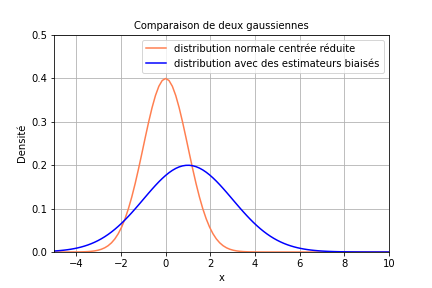
\includegraphics[width = .7\textwidth]{normal_distribution.png}
%\label{fig:1.15}
% This is a label we can use to reference this figure... more helpful if you have lots of figures in your proof.
\caption{La courbe bleue estime (mal) la orange par des paramètres biaisés.}
\end{figure}


\newpage

\emph{Exemple.} Considérons maintenant un jeu de données très simple qui conserve les propriétés nécessaires d'un modèle linéaire mixte. On suppose que nous avons quatre points, deux proviennent de l'individu 1 ($Ind = 1$), et les deux autres de l'individu 2 ($Ind = 2$). La variable d'intêret est $Resp$. Pour chacun des individus, les deux données sont associées aux modalités "traités" ($Treat = 0$) et "non traitées" ($Treat = 1$) : 

\vspace{4mm}

\begin{table}[h!]
        \centering
        \begin{tabular}{| c | c | c|}
        \hline
        \begin{bf} Ind \end{bf} &
        \begin{bf} Resp \end{bf} &
        \begin{bf} Treat \end{bf} \\
        \hline
        1 &  10 & 0\\
        1 & 25 & 1 \\
        2 & 3 & 0 \\
        2 &  6 & 1\\
        \hline
        \end{tabular}
\caption{Jeu de données décrit précédemment}
\end{table}

\vspace{4mm}

\emph{Remarque.} L'ensemble du code utilisé pour cet article se trouve dans le répertoire Github du projet.

\begin{figure}[H]
\centering
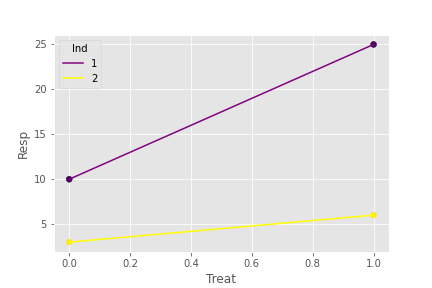
\includegraphics[width = 0.8\textwidth]{points.png}
%\label{fig:1.15}
% This is a label we can use to reference this figure... more helpful if you have lots of figures in your proof.
\caption{Représentation graphique du jeu de données}
\end{figure}

\vspace{4mm}

Si on étudie l'effet des variables $Treat$ et $Ind$ sur la variable $Resp$, on peut constuire un modèle linéaire mixte ($LMM$): 

$$Y_{Resp}= \beta X_{Treat} + \alpha K_{Ind} + \epsilon \ \ \ (0) $$

Le traitement est modélisé comme un effet fixe tandis que les effets individuels comme un effet aléatoire. On suppose que l'effet fixe n'a pas d'erreur associée mais que l'effet aléatoire en a et suit une loi normale $N(0,\sigma_s^2I)$. Enfin l'erreur résiduelle $\epsilon$ suit également une loi normale $N(0, \sigma^2I)$.\\
On peut également réaliser une régression linéaire des moindres carrés ($OLS$) pour étudier l'effet de la variable $Treat$ uniquement.


\vspace{4mm}

\begin{figure}[H]
\centering
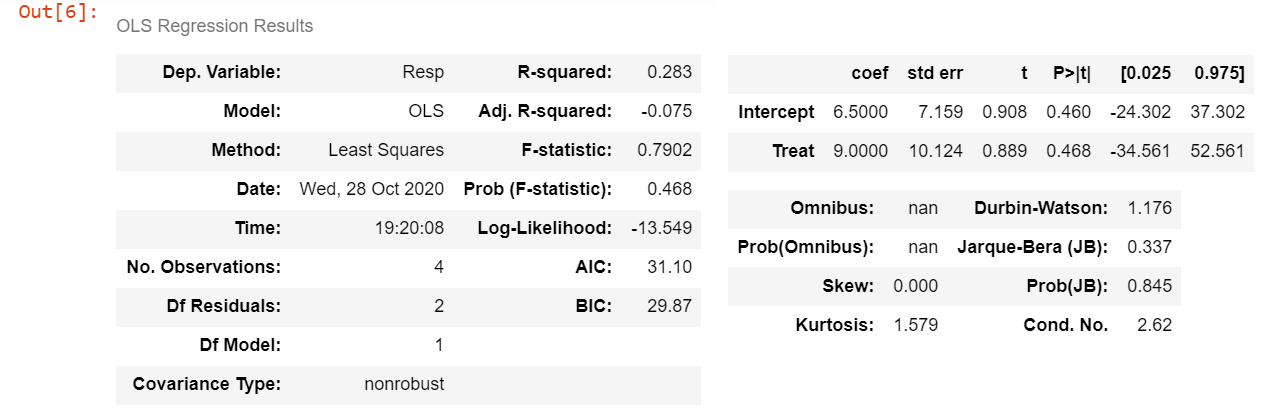
\includegraphics[width = 1\textwidth]{sortie OLS.png}
%\label{fig:1.15}
% This is a label we can use to reference this figure... more helpful if you have lots of figures in your proof.
\caption{Résultats obtenus par le modèle linéaire pour l'estimateur ML}
\end{figure}


\begin{figure}[h]

\begin{subfigure}{0.5\textwidth}
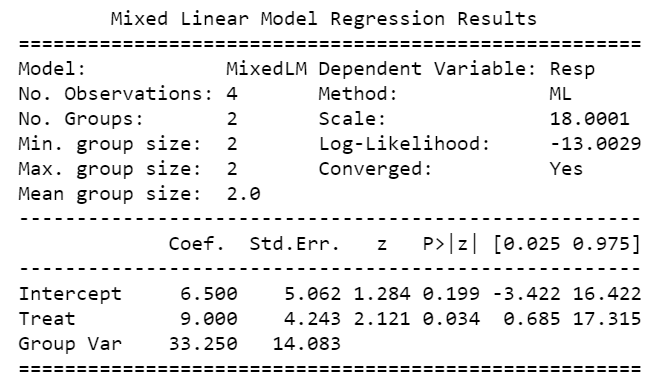
\includegraphics[width=0.9\linewidth, height=5cm]{sortie ML.png} 
\caption{Résultats pour ML}
\label{fig:subim1}
\end{subfigure}
\begin{subfigure}{0.5\textwidth}
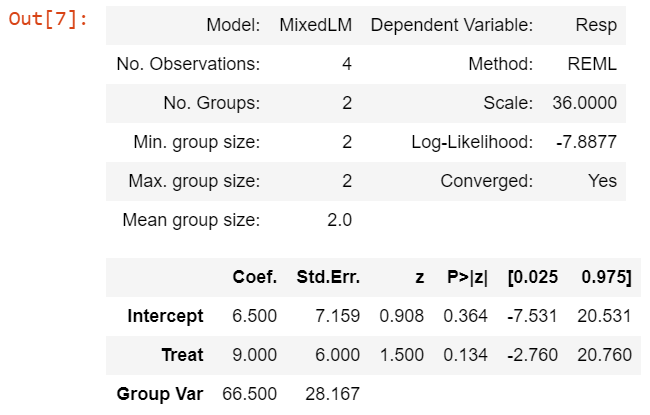
\includegraphics[width=0.9\linewidth, height=5cm]{sortie REML.png}
\caption{Résultats pour REML}
\label{fig:subim2}
\end{subfigure}

\caption{Résultats obtenus par le modèle linéaire mixte pour les deux estimateurs}
\label{fig:image2}
\end{figure}

On a donc constitué trois modèles :

\begin{enumerate}
    \item Un modèle linéaire
    \item Un modèle linéaire mixte avec estimateur du maximum de vraisemblance
    \item Un modèle linéaire mixte avec estimateur du maximum de vraisemblance restreint
\end{enumerate}

On constate déjà que que la valeur de la log-vraisemblance diffère entre les deux premiers modèles et le dernier avec une valeur de -13.5 contre -7.9. Les valeurs des coefficients de l'intercepte et de la variable $Treat$ sont les mêmes mais les intervalles de confiances diffèrent selon les modèles. Enfin en fonction de l'estimateur utilisé pour les modèles linéaires mixtes le coefficient associé à la variable de groupe est différent.\\
Notons que les 4 points ne sont pas indépendants et que l'utilisation d'une régression des moindres carrés n'est pas pertinente ni adaptée aux données. Le modèle linéaire mixte prend en compte la dépendance des données pour chaque individu.

\vspace{4mm}

Finalement, la question que l'on peut se poser ici concerne la différence entre les deux estimateurs $\rm{ML}$ et $\rm{REML}$.


\section{Les limites de l'estimateur du maximum de vraisemblance}

Dans cette partie nous allons soulever le problème essentiel de l'estimateur du maximum de vraisemblance de la variance. Ce dernier se calcule à partir de l'estimation de la moyenne qui peut avoir une erreur, ce qui entraîne un biais conséquent.

\vspace{4mm}

\emph{Proposition.} L'estimateur du maximum de vraisemblance (ML) de $\sigma^2$ est biaisé.

\vspace{4mm}

Considérons le cas simple à une dimension pour démontrer que l'estimateur du maximum de vraisemblance de la variance est biaisé. Soit $y = (y_1, y_2, ..., y_N)$ suivant une loi normale centrée réduite, avec $N$ le nombre d'observations. La vraisemblance de ce modèle est :  

$$
L(\hat{\mu},\hat{\sigma}^2)=\prod_{i=1}^N{\frac{1}{\sqrt{2\pi \hat{\sigma}^2}}}\rm{\large e}^{\displaystyle -\frac{\displaystyle (y_i-\hat{\mu})^2}{\displaystyle 2\hat{\sigma}^2}}
$$

avec $\hat{\mu}$ l'estimateur de la moyenne $\mu$, et $\hat{\sigma}^2$ l'estimateur de la variance. On choisit de travailler avec la log-vraisemblance par souci de simplicité des calculs de dérivation :

$$
l(\hat{\mu},\hat{\sigma}^2)=\log\left(L(\hat{\mu},\hat{\sigma}^2)\right)=-\frac{N}{2}\log(2\pi)-\frac{N}{2}\log(\hat{\sigma}^2)-\frac{\displaystyle \sum_{i=1}^N(y_i-\hat{\mu})^2}{\displaystyle 2\hat{\sigma}^2}
$$

Pour établir les équations de vraisemblance, on calcule à partir de la log-vraisemblance les dérivées du premier ordre par rapport à $\hat{\mu}$ et $\hat{\sigma^2}$:



    $$\frac{\partial{l(\hat{\mu},\hat{\sigma}^2)}}{\partial\hat{\mu}}=\frac{\displaystyle\sum_{i=1}^N(y_i-\hat{\mu})}{\displaystyle 2\hat{\sigma}^2}=0 \ \ \ (1)$$
    $$(1) \ \ \Leftrightarrow \sum_{i=1}^N{y_i}-\hat{\mu}N=0 \ \Leftrightarrow \hat{\mu}=\frac{1}{N}\sum_{i=1}^N{y_i}$$


    $$\frac{\partial{l(\hat{\mu},\hat{\sigma}^2)}}{\partial\hat{\sigma}^2}=-\frac{N}{2\hat{\sigma}^2}+\frac{1}{2(\hat{\sigma}^2)^2}\sum_{i=1}^N(y_i-\hat{\mu})^2=0 \ \ \ (2)$$
    
    $$(2) \Leftrightarrow \frac{\partial{l(\hat{\mu},\hat{\sigma}^2)}}{\partial\hat{\sigma}^2}=-\frac{N}{2\hat{\sigma}^2}+\frac{1}{2(\hat{\sigma}^2)^2}\sum_{i=1}^N(y_i-\hat{\mu})^2=0$$
    $$(2) \Leftrightarrow N=\frac{1}{\hat{\sigma}^2}\sum_{i=1}^N(y_i-\hat{\mu})^2 \Leftrightarrow
    \hat{\sigma}^2=\frac{1}{N}\sum_{i=1}^N(y_i-\hat{\mu})^2$$

\vspace{4mm}

Soit $\mu$ la vraie valeur de la moyenne. La valeur attendue de $\sigma^2$ est donc:

$$\sigma^2\equiv\rm{Var}(y)=\frac{1}{N}\sum_{i=1}^N(y_i-\mu)^2$$

Toutefois, si on restructure l'expression de $\hat{\sigma^2}$, on a:

\vspace{2mm}

$\hat{\sigma}^2=\frac{1}{N}\sum_{i=1}^N(y_i-\hat{\mu})^2=\frac{1}{N}\sum_{i=1}^N\left[(y_i-\mu)-(\hat{\mu}-\mu)\right]^2$

$\hat{\sigma}^2=\frac{1}{N}\sum_{i=1}^N(y_i-\mu)^2-\frac{2}{N}\sum_{i=1}^N(y_i-\mu)(\hat{\mu}-\mu)+ \frac{1}{N}\sum_{i=1}^N(\hat{\mu}-\mu)^$

$\hat{\sigma}^2=\frac{1}{N}\sum_{i=1}^N(y_i-\mu)^2-\frac{2(\hat{\mu}-\mu)}{N}\sum_{i=1}^N(y_i-\mu)+(\hat{\mu}-\mu)^2
$

\vspace{4mm}

D'autre part on exprime le terme $\sum_{i=1}^N(y_i-\mu)$ en fontion de $\hat{\mu}$: 

$$\hat{\mu}-\mu=\frac{1}{N}\sum_{i=1}^N{y_i}-\mu=\frac{1}{N}\sum_{i=1}^N{y_i}-\frac{1}{N}\sum_{i=1}^N{\mu}=\frac{1}{N}\sum_{i=1}^N{(y_i-\mu)}\ \ \ (3)$$
$$(3) \Rightarrow \sum_{i=1}^N{(y_i-\mu)}=N(\hat{\mu}-\mu)$$

\vspace{4mm}

Enfin on remplace l'expression de $\sum_{i=1}^N(y_i-\mu)$ obtenue dans la formule de l'estimateur du maximum de vraisemblance de la variance: 
$$
\hat{\sigma}^2=\frac{1}{N}\sum_{i=1}^N(y_i-\mu)^2-\frac{2(\hat{\mu}-\mu)}{N}N(\hat{\mu}-\mu)+(\hat{\mu}-\mu)^2=\frac{1}{N}\sum_{i=1}^N(y_i-\mu)^2-(\hat{\mu}-\mu)^2
$$

On calcule à partir de cette expression le biais de $\hat{\sigma^2}$, sachant qu'on connaît l'expression théorique de la variance $\sigma^2$ attendue:


$E[\hat{\sigma}^2]=E\left[\frac{1}{N}\sum_{i=1}^N(y_i-\mu)^2\right]-E[(\hat{\mu}-\mu)^2]=\sigma^2-E[(\hat{\mu}-\mu)^2]$

$E[\hat{\sigma}^2]=\sigma^2-\rm{Var}(\hat{\mu})=\sigma^2-\rm{Var}\left(\frac{1}{N}\sum_{i=1}^N{y_i}\right)=\sigma^2-\frac{1}{N^2}\sum_{i=1}^N{\rm{Var}(y_i)}$

$E[\hat{\sigma}^2]=\sigma^2-\frac{1}{N^2}N\sigma^2=\sigma^2-\frac{\sigma^2}{N}=\frac{N-1}{N}\sigma^2$

\vspace{4mm}

On constate que l'espérance de l'estimateur $\rm{ML}$ de la variance n'est pas égale à la variance $\sigma^2$. L'estimateur $\rm{ML}$  sous-estime la vraie variance.\\
En revanche, la différence entre la variance réelle et la variance estimée devient plus petite pour de grands échantillons.\\ 
Cependant, nous avons considéré ici le cas unidimensionnel le plus simple. Lorsque $ Y $ n'est pas un vecteur mais une matrice, c'est-à-dire pour des données de grande dimension, il peut être montré que l'expression précédente prend la forme :

$$
E[\hat{\sigma}^2]=\frac{N-k}{N}\sigma^2
$$

où $k$ est le nombre de dimensions. Par conséquent, le problème de la sous-estimation de la vraie variance par $\rm{ML}$ devient particulièrement aigu, et l'estimateur de variance $\rm{ML}$ devient de plus en plus biaisé lorsque le nombre de dimensions $ k $ se rapproche du nombre d'observations $ N $. Ici, nous voyons clairement que dans un espace de grande dimension, le principe du maximum de vraisemblance $\rm{ML}$ ne fonctionne bien que dans la limite $ k << N $, tandis que des résultats biaisés peuvent être trouvés lorsque $ k \approx N $.

\section{L'estimateur REML, une solution au problème de biais}

L'incertitude sur l'estimateur de la variance vient du fait que celui-ci est calculé à partir de l'estimateur de la moyenne. Notre stratégie ici va être d'exprimer la log-vraisemblance sans aucune information sur la moyenne. Un moyen de se passer des informations sur la moyenne de la fonction log-vraisemblance est de calculer une probabilité marginale, c'est-à-dire d'intégrer la log-vraisemblance sur la moyenne. Ici, nous allons intégrer la log-vraisemblance par rapport à $\beta$ et obtenir une estimation sans biais pour les composantes de la variance.

\vspace{4mm}

On se place ici dans un espace de dimension $k=2$, dans le contexte du modèle linéaire mixte $(0)$ exposé dans la première partie dans l'exemple où, on le rappelle, $\sigma^2$ est la variance de l'erreur résiduelle et $\sigma^2_s$ celle de l'effet aléatoire. On a alors $ Y \sim N(X\beta, \Sigma_y)$ où $\Sigma_y$ vaut:

\[ \Sigma_y = \begin{pmatrix} \sigma^2+\sigma_s^2 & \sigma_s^2 & 0 & 0 \\ \sigma_s^2 & \sigma_s^2+\sigma^2 & 0 & 0 \\ 0 & 0 & \sigma^2+\sigma_s^2 & \sigma_s^2 \\ 0 & 0 & \sigma_s^2 & \sigma_s^2+\sigma^2 \end{pmatrix}\]

\vspace{4mm}

La vraisemblance du modèle, relative à une distribution gaussienne multivariée est:

\[L(\beta, \sigma_s^2, \sigma^2) = \frac{1}{\sqrt{2\pi |\Sigma_y|}}e^{-\frac{\trans{(Y-X\beta)}\Sigma_y^{-1}(Y-X\beta)}{2}}\]

\vspace{4mm}

On intègre cette vraisemblance par rapport à $\beta$ pour calculer la "log-vraisemblance":

$$l=log\left[\int L(\beta, \Sigma_y) \ d\beta\right] = -\frac{1}{2}log(2\pi)-\frac{1}{2}log(|\Sigma_y|)+log\left[\int e^{-\frac{\trans{(Y-X\beta)}\Sigma_y^{-1}(Y-X\beta)}{2}} d\beta\right]$$

\vspace{4mm}

On utilise l'approche du point de selle. La fonction exponentielle sous l'intégrale décroît très rapidement, il suffit donc de calculer l'intégrale pour le minimum de la fonction $f(\beta)$ où:

$$f(\beta)=\frac{\trans{(Y-X\beta)}\Sigma_y^{-1}(Y-X\beta)}{2}$$ 

qui donnera une contribution maximale à l'exposant de l'exponentielle et donc à la log-vraisemblance. 

\vspace{4mm}

On obtient par un développement de Taylor: $f(\beta)\approx f(\hat{\beta})+(1/2)(\beta-\hat{\beta})^2f''(\hat{\beta})$. Ce développement se fait au point $\hat{\beta}$, l'estimateur \rm{ML} de $\beta$. On suppose que $\hat{\beta}$ est assez proche de la vraie valeur de $\beta$ de sorte que la vraisemblance soit maximale et que l'on puisse réaliser ce développement. On obtient:

$$
f(\beta)=-\frac{\displaystyle \left(Y-X\beta\right)^T\Sigma_y^{-1}\left(Y-X\beta\right)}{\displaystyle 2}\approx-\frac{\displaystyle \left(Y-X\hat{\beta}\right)^T\Sigma_y^{-1}\left(Y-X\hat{\beta}\right)}{\displaystyle 2}-\frac{\displaystyle \left(\beta-\hat{\beta}\right)^TX^T\Sigma_y^{-1}X\left(\beta-\hat{\beta}\right)}{\displaystyle 2}
$$

Finalement, en réinjectant cette expression dans celle de la log-vraisemblance, on a: 

$$l = -\frac{1}{2}\log{\left(2\pi\right)} - \frac{1}{2}\log{\left(\lvert\Sigma_y\rvert\right)}-\frac{\displaystyle \left(Y-X\hat{\beta}\right)^T\Sigma_y^{-1}\left(Y-X\hat{\beta}\right)}{\displaystyle 2}+\log\left[\int\rm{\large e}^{-\frac{\displaystyle \left(\beta-\hat{\beta}\right)^TX^T\Sigma_y^{-1}X\left(\beta-\hat{\beta}\right)}{\displaystyle 2}} d\beta \right]$$

$$l= \log\left[\int\rm{\large L}(\beta, \Sigma_y)d\beta\right] =- \frac{1}{2}\log{\left(\lvert\Sigma_y\rvert\right)}-\frac{1}{2}\displaystyle \left(Y-X\hat{\beta}\right)^T\Sigma_y^{-1}\left(Y-X\hat{\beta}\right)-\frac{1}{2}\log\left(|X^T\Sigma_y^{-1}X|\right)$$

On reconnaît dans les premiers termes l'expression de la log-vraisemblance du modèle linéaire mixte pour $k>1$. Le dernier terme $-\frac{1}{2}\log\left(|X^T\Sigma_y^{-1}X|\right)$ est issu de l'approximation $\rm{REML}$ et semble constituer le biais dans l'estimation $\rm{ML}$ classique.

\vspace{4mm}

\emph{Exemple.} Revenons au petit jeu de données présenté précédemment en partie $1$. Le modèle linéaire mixte sous forme matricielle qui lui est associé est le suivant: 

\begin{equation}
\label{eq:matrix_eqs}
\begin{aligned}
\begin{bmatrix}
y_{11} \\
y_{21} \\
y_{12} \\
y_{22}
\end{bmatrix} = 
\begin{bmatrix}
1 & 0 \\
0 & 1 \\
1 & 0 \\
0 & 1
\end{bmatrix}
\begin{bmatrix}
\beta_1 \\
\beta_2
\end{bmatrix}+
\begin{bmatrix}
1 & 0 \\
1 & 0 \\
0 & 1 \\
0 & 1
\end{bmatrix}
\begin{bmatrix}
\alpha_1 \\
\alpha_2
\end{bmatrix}+
\begin{bmatrix}
\epsilon_{11} \\
\epsilon_{21} \\
\epsilon_{12} \\
\epsilon_{22}
\end{bmatrix}
\end{aligned}
\end{equation}

avec $(y_{11},y_{21}, y_{12}, y_{22})=(3, 6, 10, 25)$.

On va estimer la matrice de variances-covariances de ce modèle à partir des formules établies précédemment. On se sert des valeurs de $(\beta_1,\beta_2)=(6.5, 15.5)$ communes aux trois modèles construits dans la partie $1$. On a également besoin des expressions suivantes pour le calcul de la vraisemblance: 

\vspace{2mm}

$
\lvert\Sigma_y\rvert = 4\sigma_s^4 \sigma^4 + 4\sigma_s^2 \sigma_s^6 + \sigma^8
$

\vspace{2mm}

$
\left(Y-X\beta\right)^T\Sigma_y^{-1}\left(Y-X\beta\right) = \frac{1}{\sigma^2(\sigma^2+2\sigma_s^2)}\left[(y_{11}-\beta_1)^2(\sigma^2+\sigma_s^2) - 2(y_{11}-\beta_1)(y_{21}-\beta_2)\sigma_s^2 + \right. \\ 
\left. (y_{21}-\beta_2)^2(\sigma^2+\sigma_s^2) + (y_{12}-\beta_1)^2(\sigma^2+\sigma_s^2) - 2(y_{12}-\beta_1)(y_{22}-\beta_2)\sigma_s^2 + (y_{22}-\beta_2)^2(\sigma^2+\sigma_s^2) \right]
$

\vspace{2mm}

$
|X^T\sigma_y^{-1}X|=\frac{4}{\sigma^2(\sigma^2+2\sigma_s^2)}
$

\vspace{4mm}

On trouve en maximisant l'expression de la log-vraisemblance approchée (voir Illustrations.py): $\sigma^2=6$ et $\sigma^2_s=8.15$ qui donnent à la log-vraisemblance la valeur maximale de $-6.049856$. Dans la partie 1 (voir figure $4.b$), on trouvait les mêmes valeurs pour les estimateurs $\rm{REML}$ de la variance puisque $\sigma^2=\sqrt{Scale}=\sqrt{36}=6$ et $\sigma^2_s=\sqrt{Groupe \ var}=\sqrt{33.25}=8.15$.

\begin{thebibliography}{}
\bibitem{}Nikolay Oskolkov, Maximum Likelihood (ML) vs. Restricted Maximum Likelihood (REML), https://towardsdatascience.com/maximum-likelihood-ml-vs-reml-78cf79bef2cf, 2020
\bibitem{}Mégane Diéval, Maximum de vraisemblance vs. Maximum de vraisemblance restreint https://github.com/MegDie/ML\_VS\_REML, 2020
\bibitem{}Joseph Salmon. HMMA307 - Modèles linéaires avancés, 2020

\end{thebibliography}

















\end{document}